\documentclass[sigplan,screen]{acmart}
\def\BibTeX{{\rm B\kern-.05em{\sc i\kern-.025em b}\kern-.08emT\kern-.1667em\lower.7ex\hbox{E}\kern-.125emX}}

\copyrightyear{2018}
\acmYear{2018}
\setcopyright{acmlicensed}
\acmConference[Woodstock '18]{Woodstock '18: ACM Symposium on Neural Gaze Detection}{June 03--05, 2018}{Woodstock, NY}
\acmBooktitle{Woodstock '18: ACM Symposium on Neural Gaze Detection, June 03--05, 2018, Woodstock, NY}
\acmPrice{15.00}
\acmDOI{10.1145/1122445.1122456}
\acmISBN{978-1-4503-9999-9/18/06}

\usepackage{times}
\usepackage{graphicx}
\usepackage{url,hyperref}


\begin{document}

\title{Assignment 1}

\author{Joshua Drumm}
\email{jkdrumm@asu.edu}
\affiliation{%
	\institution{Arizona State University}
}

\author{Jainish Soni}
\email{jjsoni@asu.edu}
\affiliation{%
	\institution{Arizona State University}
}

\date{\today}

\begin{abstract}
Working with multiple agile teams presents new problems compared to working with a single agile team. To overcome these new problems, new techniques and positions can be used. While additional communication is important, so is a new structure. Having the software architecture and design well known throughout all teams is vital for success.
\end{abstract}
\maketitle

\newpage
\pagenumbering{arabic}


%\keywords{}

\section{Introduction}
As projects become larger and larger, there becomes a need for more people to complete them. However, scaling agile is not very straight forward. With enough people on one project, there can be many different agile teams all working together. In order to effectively deliver a successful product, there are some additional agile techniques that should be employed by anyone using multiple agile teams.

\section{Questions}

\subsection{Question-1}
Type here

\subsubsection{figure}
	\begin{figure}[h]
	\end{figure}

\subsection{Question-2}
While having a plan to follow is already important enough in software engineering, it is even more important when working with multiple agile teams. In order for teams to stay focused on the goal, the architecture and design must be fully understood across all teams.
In order to achieve this with large or multiple teams, it is important to have an architecture owner in order to avoid conflicts between developers and between teams. This can be an additional role in scrum much like the product owner and the scrum master. While the architecture owner has the ultimate power to influence the direction of the architecture, they should still work with the developers in order to create an architectural environment that the developers can work in easily. \cite{WAmbler} This role is important because without an architecture owner, many developers can disagree on the design of a project. Having an architecture owner can help bring people to agreement, always having the final decision. \par
When dealing with especially large agile teams, it can be beneficial to have a separate team of architecture owners. There would be an architecture owner for each other team, and there would also be a chief architecture owner to oversee the other architecture owners \cite{WAmbler}. The structure for this style of system is visualized in Figure \ref{fig:label1} When using a system like this, there are four approaches to creating the teams: architecture-driven, feature-driven, open source, and combinational. \cite{WAmbler} \par
In order to follow an architectural plan with many agile teams, it is important to have a good model of the architecture. The models do not need to be very detailed, but must be understood by every team.

\begin{figure}[!htb]
        \center{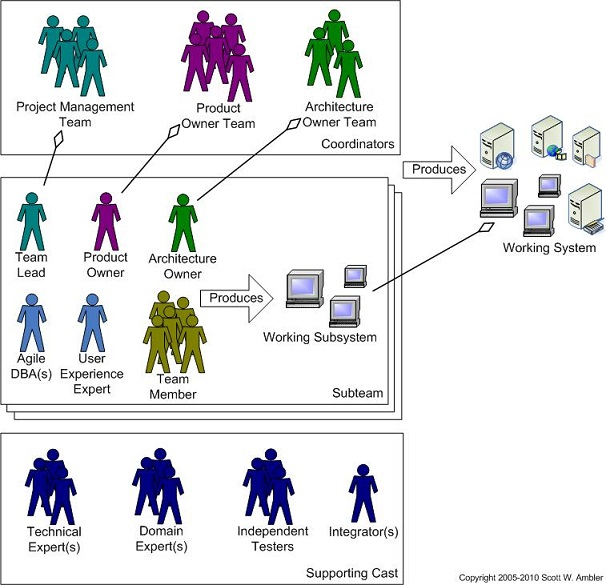
\includegraphics[scale=0.5]{agileTeamLarge.jpg}}
        \caption{\label{fig:label1} How to divide and structure architecture owners among teams \cite{WAmbler}}
\end{figure}


\subsubsection{figure}
	\begin{figure}[h]
	\end{figure}

\section{Conclusion}
The results are here. Referring to section \ref{sec1} on page \pageref{sec1}

\newpage
\nocite{*} %Remove this in the future. This allows for things not being cited to be present
\bibliographystyle{ACM-Reference-Format}
\bibliography{Assignment1References}

\end{document}